% Polycopie pour les etudiants

%\documentclass[handout]{beamer}[10pt, usepdftitle=false]
%%\usepackage[printwatermark]{xwatermark}
%usepackage{pgfpages}
%\pgfpagesuselayout{6 on 1}[a4paper,border shrink=5mm] % 4 par 4

% NE PAS OUBLIER DE BAISSER A QUALITE DU POLYCOPIE!: gs -sDEVICE=pdfwrite -dCompatibilityLevel=1.4 -dPDFSETTINGS=/ebook -dNOPAUSE -dQUIET -dBATCH -sOutputFile=small.pdf big.pdf

% Mes slides pour le cours
\documentclass{beamer}[10pt, usepdftitle=false handout]

\beamertemplatenavigationsymbolsempty

\usepackage[T1]{fontenc}
\usepackage[]{algorithm2e}
\usepackage{multimedia}
\usepackage{gensymb}
\usepackage{textcomp}
\usepackage{array}
\usepackage{fancyvrb}
\usepackage{tabularx,colortbl}

\usepackage{listings}

%\usepackage{background}
%\backgroundsetup{
%    placement=center,
%    scale=5,
%    color=lightgray,
%    contents={PAUL BLONDEL},
%    opacity=0.5
%}
%\setbeamertemplate{background}{\BgMaterial}


%\usepackage[font=small,labelfont=bf]{caption} 

\usetheme{Boadilla}

\title{Introducton to Data Engineering 8}
\author[]{Paul Blondel}
\institute[]{UTSEUS, Shanghai}
\date[]{March 30st, 2021}

\usepackage[style=british]{csquotes}


\def\signed #1{{\leavevmode\unskip\nobreak\hfil\penalty50\hskip1em
  \hbox{}\nobreak\hfill #1%
  \parfillskip=0pt \finalhyphendemerits=0 \endgraf}}

\newsavebox\mybox
\newenvironment{aquote}[1]
  {\savebox\mybox{#1}\begin{quote}\openautoquote\hspace*{-.7ex}}
  {\unskip\closeautoquote\vspace*{1mm}\signed{\usebox\mybox}\end{quote}}


\setbeamertemplate{headline}
{
  \leavevmode%
  \hbox{%
  \begin{beamercolorbox}[wd=1.0\paperwidth,ht=2.25ex,dp=1ex,center]{author in head/foot}%
    \usebeamerfont{author in head/foot}\insertsubsection
  \end{beamercolorbox}}%
  \vskip0pt%
}


\setbeamertemplate{footline}
{
  \leavevmode%
  \hbox{%
  \begin{beamercolorbox}[wd=.5\paperwidth,ht=2.25ex,dp=1ex,center]{author in head/foot}%
    \usebeamerfont{author in head/foot}\insertsection
  \end{beamercolorbox}%
  \begin{beamercolorbox}[wd=.5\paperwidth,ht=2.25ex,dp=1ex,center]{title in head/foot}%
    \usebeamerfont{title in head/foot} \inserttitle \hspace*{2em}  \insertframenumber{} / \inserttotalframenumber\hspace*{2ex} 
  \end{beamercolorbox}}%
  \vskip0pt%
}

\AtBeginSection[]
{
   \begin{frame}
    \tableofcontents[ 
    currentsection] 
   \end{frame}
}

\begin{document}
	{
	\setbeamertemplate{footline}{
  	\leavevmode%
  	\hbox{%
  	\begin{beamercolorbox}[wd=.5\paperwidth,ht=2.25ex,dp=1ex,center]{author in head/foot}%
  	\end{beamercolorbox}%
  	\begin{beamercolorbox}[wd=.5\paperwidth,ht=2.25ex,dp=1ex,center]{title in head/foot}%
  	\end{beamercolorbox}}%
  	\vskip0pt%	
	} 
	\begin{frame}
	\titlepage
	\end{frame}

	\begin{frame}
	
	\begin{aquote}{Eric Schmidt, PDG Google, 2010}
There was 5 exabytes of information created between the
dawn of civilization through 2003, but that much information
is now created every 2 days, and the pace is increasing.
	\end{aquote}	
	\end{frame}

	\begin{frame}
		\tableofcontents
	\end{frame}
	}

	\addtocounter{framenumber}{-3}

	\section{What is Big Data?}	

    \begin{frame}[label=(first)]
	
	What is Big Data?	
	\vspace*{0.6em}
	
Big Data refers to \textbf{datasets that become so large, so various and changing so rapidly} that they are difficult to work with using traditional database management or information management tools.

	\begin{figure}
		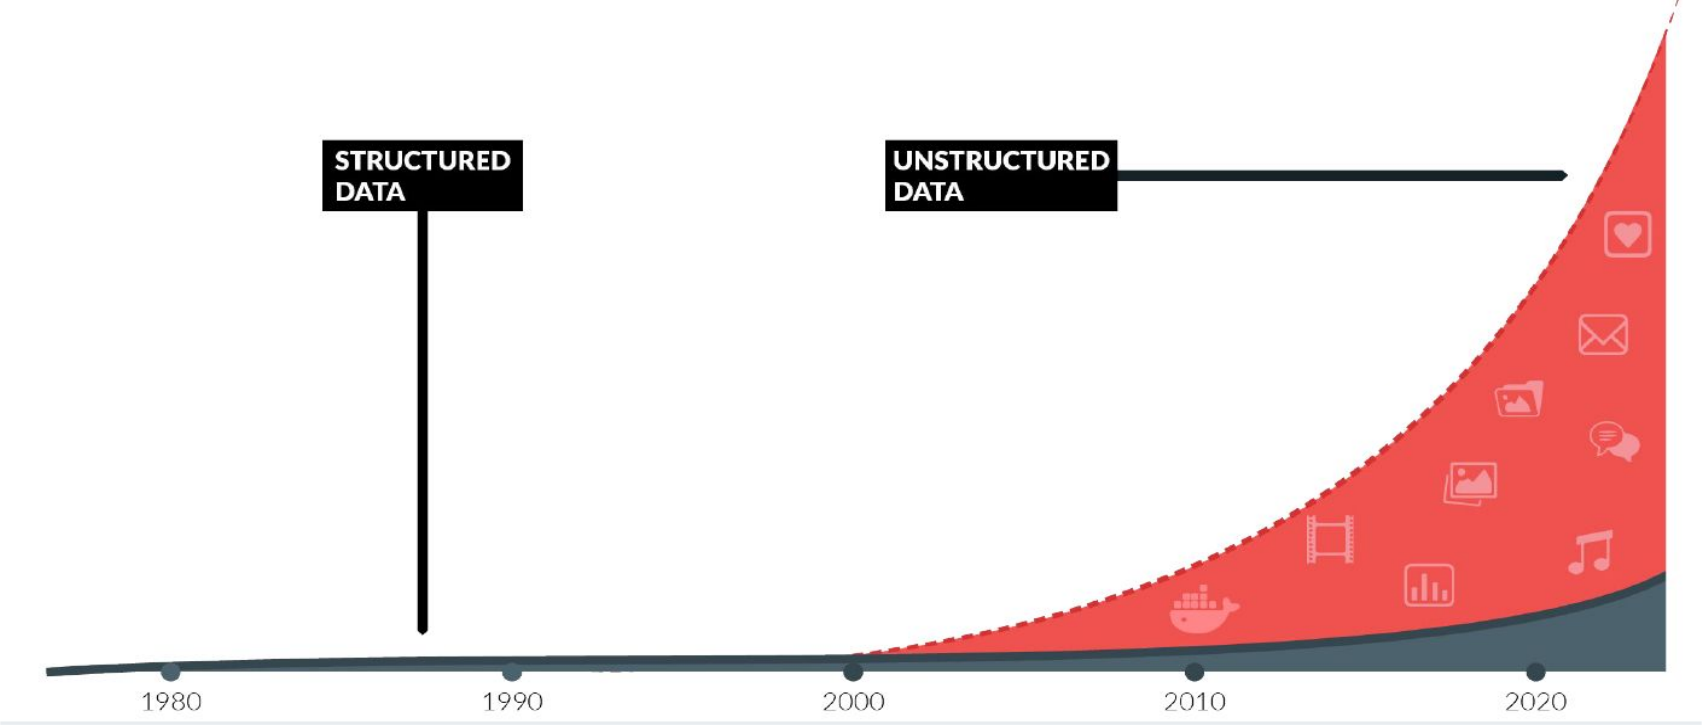
\includegraphics[scale=0.8]{images/expo-growth-big-data.png} 
     	\vspace*{-0.5em}
		\caption{Exponential growth of data in the recent years}
	\end{figure}		
	
	\end{frame}

	\begin{frame}
	
	When refering to Big Data it is common to talk about the three Vs: \textbf{high Volume} of data, \textbf{high Velocity} of data input and \textbf{high Variety} of data (structured+unstructured):
	\vspace*{0.6em}
	
	\begin{figure}
	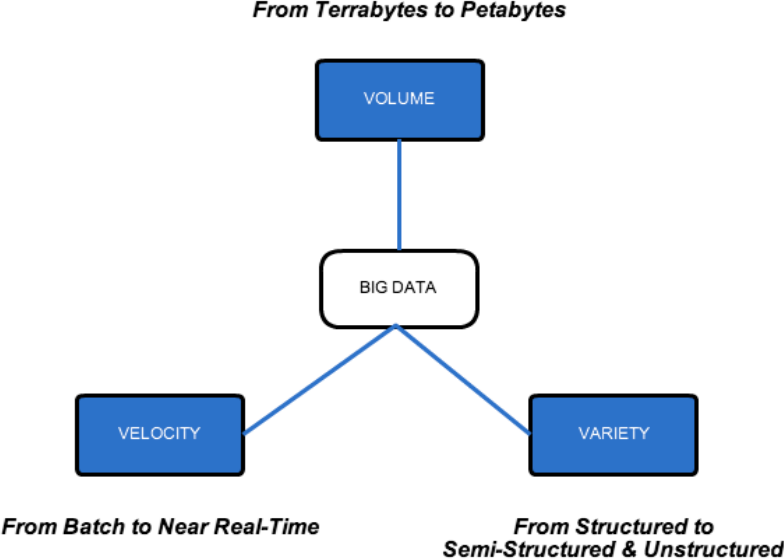
\includegraphics[scale=1.2]{images/three-v.png} 
     	\vspace*{-0.5em}
		\caption{The three Vs.}
	\end{figure}

	
	
	\end{frame}

	\begin{frame}
	
	\begin{itemize}

	\item{\textbf{High Volume}:
		\begin{itemize}
		\item{Data cannot fit anymore inside one server (Ex: Facebook in 2018: 7 Petabytes (10E15) of new data per day}
		\item{Exponential trend: 90\% of the total data created was created in the last two years!}		
				
		\end{itemize}
		}	
	\item{\textbf{High Velocity}:
		\begin{itemize}
			\item{Increasing flows of data need to be analyzed  (ex: stock market inform, user behavior of e-commerce website)}
			\item{Information needs more and more to be analyzed in near real-time}		
		\end{itemize}			
	
	}
	
	\item{\textbf{High Variety}:
	
	\begin{itemize}
		\item{Data can be raw, semi-structured or even unstructured (Ex: text, images, videos, metadata, computer code etc.)}	
	\end{itemize}
	
	}	
	\end{itemize}		
	
	
	\end{frame}	
	
	\begin{frame}
	
	Structured VS unstructured data, what is the difference?
	\vspace*{0.6em}
	
	\begin{itemize}
		\item{\textbf{Structured data}: information (words, signs, numbers...) controlled by repositories and presented in boxes (fields of a database) allowing their interpretation and processing by computers}
		
		\item{\textbf{Unstructured data}: the rest, everything that is not organized in a database (email, images, videos, etc.)}	
	\end{itemize}		
	

		
	\end{frame}	
	
	\section{Hadoop}	
	
	
	\begin{frame}
	

	\begin{itemize}
		\item{Processing such large amounts of data \textbf{requires a new paradigm}...}
		\item{Indeed, a single server machine, even a high-end one is unable to process so much information}
	\end{itemize}
	
	\begin{block}{Solution}
	Distribute the data on several server machines and use massive parallel calculation and distributed storage with Hadoop technology
	\end{block}	

	\begin{figure}
	
\includegraphics[scale=0.3]{images/hadoop_logo.png} 
	\end{figure}			
	
	\end{frame}	
	
	
	\begin{frame}
	
	\textbf{Before Big Data}: adding memory and CPU power permitted to \textbf{scale vertically} a server capacity	
	\vspace*{0.6em}	


	\begin{figure}
	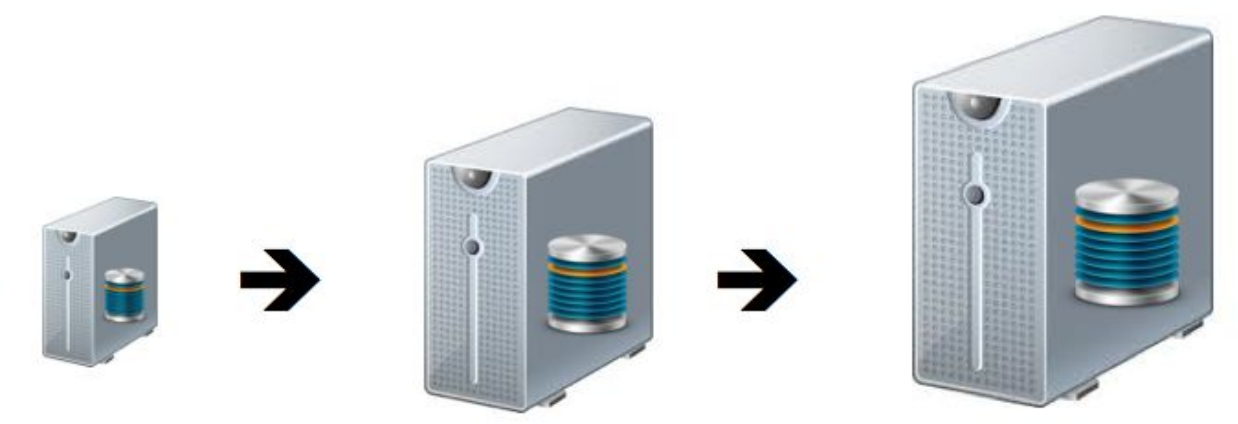
\includegraphics[scale=0.3]{images/vertical-scaling.png} 
     	\vspace*{-0.5em}
		\caption{Vertical scaling}
	\end{figure}	
	
	However this approach has a \textbf{lot of limitations when dealing with Big Data}... To deal with Big Data, you have to \textbf{horizontally scale} a cluster of machines which is easier to scale and more robust:
	\vspace{0.6em}		
	
	\begin{figure}
	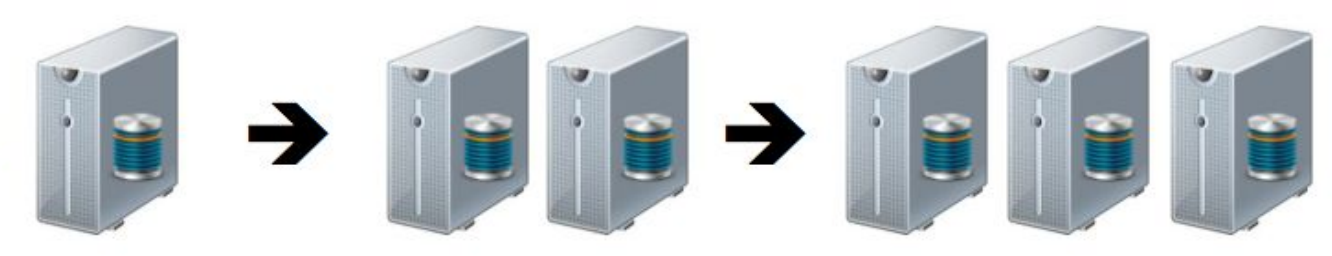
\includegraphics[scale=0.3]{images/horizontal-scaling.png} 
     	\vspace*{-0.5em}
		\caption{Horizontal scaling of a cluster}
	\end{figure}	
	
	\begin{block}{Cluster}
	A cluster of machines is a set of computers that work together so they \textbf{can be viewed from outside as one single system}	
	\end{block}	
	
	
	\end{frame}
	
	\begin{frame}
	A cluster of machines using Hadoop:	
	\vspace*{0.6em}
	
	\begin{figure}
	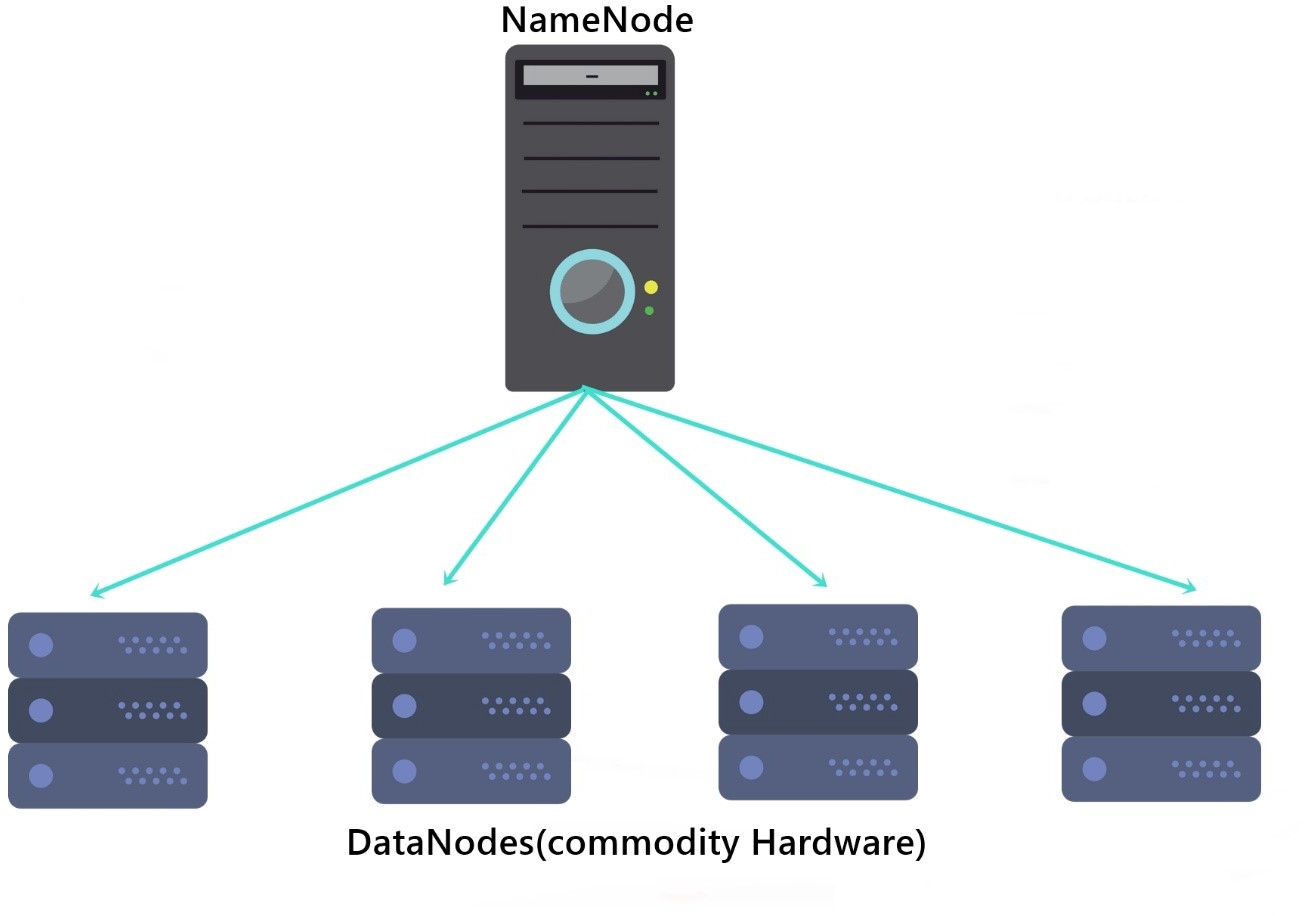
\includegraphics[scale=0.5]{images/hadoop-cluster.png} 
     	\vspace*{-0.5em}
		\caption{A Hadoop cluster made of a Namenode and Datanodes}
	\end{figure}	
			
	\begin{block}{Hadoop}
	Hadoop is a technology permitting the storage and the processing of massive amount of data on a cluster
	\end{block}	
		
	\end{frame}	
	
	\begin{frame}
	
	\begin{itemize}
	\item{\textbf{Storage with Hadoop cluster}: 
		\begin{itemize}
		\item{All the \textbf{machines are connected to each other in order to share storage space} using \textbf{HDFS}}
		\item{Ex: Cloud is an example of a distributed storage space: files are stored on different machines and duplicated}
		\end{itemize}
	}
		
	\item{\textbf{Processing with Hadoop cluster}:	
		\begin{itemize}
			\item{The execution of a program is also distributed: it is \textbf{executed on one or more machines of the cluster}}
			\item{Specifically with Hadoop: the \textbf{MapReduce paradigm} allows a cluster of computers to execute tasks in chunks in an extremely parallel manner}
		\end{itemize}
	}	
	
	\end{itemize}		
	
	\end{frame}
	
	\begin{frame}	
To store massive data on a cluster we need:
\vspace*{0.6em}

\begin{itemize}
	\item{A \textbf{special file system allowing to see only one space containing gigantic and very numerous files} (\textbf{HDFS})}
	\item{Specifically designed \textbf{databases working on cluster of machines} (HBase, Cassandra, ElasticSearch)}
\end{itemize}

To compute massive computation on a cluster we need:
\vspace*{0.6em}

\begin{itemize}
\item{A new processing paradigm:
	\begin{itemize}
		\item{This new paradigm is called \textbf{MapReduce}}
		\item{With this: \textbf{easy to parallelize executions at a massive scale}}		
	\end{itemize}}
\end{itemize}

\begin{block}{Content of the course}
We will talk about Hadoop's \textbf{HDFS} and Hadoop \textbf{MapReduce} and \textbf{Spark}	
\end{block}	
			
	\end{frame}		
	
\subsection{HDFS: designed for massive storage}	
	
	\begin{frame}
	
	\textbf{HDFS} (Hadoop Distributed File System) is the \textbf{distributed file system} (across a cluster) of Hadoop:
	\vspace{0.6em}
	
	\begin{itemize}
		\item{Inspired by "Google File System"}	
		\item{HDFS is composed of two services:
			\begin{itemize}
			\item{\textbf{Namenode}: contains all the \textbf{names and the locations of the block files} in the FS (like a big phone book)}
			\item{\textbf{Datanode}: \textbf{store the blocks of the stored files}}
			\end{itemize}}
		\item{A \textbf{file written to HDFS is divided into blocks} (64MB to 256MB each)}
		\item{\textbf{Blocks are replicated and distributed across multiple Datanodes} (usually 3x)}
		\item{The FS queries the Namenode to \textbf{learn the stucture of the file tree and find where are the blocks}}
		\item{\textbf{Clients access data directly from the Datanode}, with having this knowledge}	
	\end{itemize}
	
	
	\end{frame}
	
	\begin{frame}
	
	How HDFS read and write data in the cluster:
	\vspace*{0.6em}

	\begin{figure}
	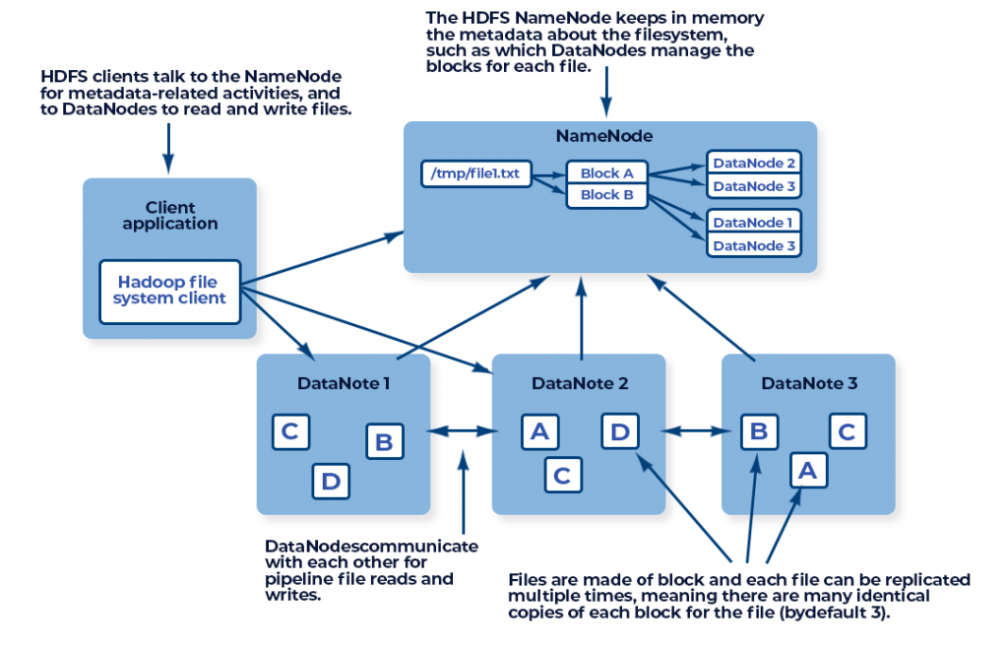
\includegraphics[scale=1.3]{images/hdfs-work.png} 
	\end{figure}	
	
	
	\end{frame}
	
	\begin{frame}
	
HDFS is a distributed file system:
\vspace*{0.6em}

\begin{itemize}
	\item{\textbf{Files and folders are organized in a tree} (like Unix)}
	\item{Files are \textbf{stored on a large number of machines} in such a way that the \textbf{exact position of files is invisible}}
	\item{\textbf{File access is transparent} whatever the machines that contain the files}
	\item{Files are copied in several copies for \textbf{robustness} and allow \textbf{multiple simultaneous accesses}}
\end{itemize}
\vspace*{0.6em}
	
HDFS \textbf{allows to see all folders and files of these thousands of machines as a single machines as a single tree} containing Po of data, as if they were on the local hard drive.	
		
	\end{frame}
	
	\begin{frame}[fragile]
	
The "\textbf{hdfs dfs}" command and its options allows to manage the files and folders:
\vspace*{0.6em}

\begin{verbatim}
hdfs dfs -help
hdfs dfs -ls [names...] (no -l option) 
hdfs dfs -cat name 
hdfs dfs -mv old new
hdfs dfs -cp old new
hdfs dfs -mkdir folder 
hdfs dfs -rm -f -r folder (no -en option)
hdfs dfs -chmod 777 /stuff
\end{verbatim}

These commands take some time to react (HDFS is slow) mainly these are programs written in Java loading a lot of Java libraries (jars). 
		
\end{frame}
\begin{frame}[fragile]
	
Commands to exchange content between HDFS and the "world":
\vspace*{0.6em}

\begin{verbatim}
hdfs dfs -copyFromLocal filesource filedestination
hdfs dfs -put filesource [filedestination] 
\end{verbatim}

To extract a file from HDFS, there are two possible commands:
\begin{verbatim}
hdfs dfs -copyToLocal filesource destination files
hdfs dfs -get filesource [filedestination]
\end{verbatim}
 
Other examples:
\begin{verbatim}
hdfs dfs -mkdir -p books
wget http://www.textfiles.com/etext/FICTION/dracula
hdfs dfs -put dracula books
hdfs dfs -ls books
hdfs dfs -get books/center_earth 
\end{verbatim}
	
\end{frame}
\begin{frame}

HDFS benefits:
\vspace*{0.6em}

\begin{itemize}
\item{HDFS is \textbf{compatible with a lots of Big Data tools} (from the Hadoop ecosystem and other)}
\item{A \textbf{highly scalable storage} model}
\item{Availability of support (Hadoop "vendors")}
\end{itemize}
\vspace*{0.6em}

HDFS disadvantages:
\vspace*{0.6em}

\begin{itemize}
	\item{Configuration is \textbf{complex and fragile}}
	\item{\textbf{Only supports replication to avoid data loss}}
	\item{\textbf{No possibility to gather clusters} of HDFS together}
	\item{The \textbf{need to query the Namenode for each read}}
	\item{\textbf{Number of blocks limited by the Namenode memory space}... }
	\item{Relatively \textbf{slow}}
\end{itemize}

\end{frame}

\subsection{Hadoop MapReduce: towards massive parallel computation}

\begin{frame}

As mentioned before, MapReduce is the paradigm to use to apply computation on massive data distributed on a Hadoop cluster.
\vspace*{0.6em}

Let's see in more details what is MapReduce ?
\vspace*{0.6em}

\begin{itemize}
	\item{Invented in 2004 by Google}
	\item{Based on a simple \textbf{Divide and Conquer} approach}
	\item{However: \textbf{not all problems can be tackled with MapReduce} (must be a parallelizable problem)}
\end{itemize}


\end{frame}

\begin{frame}

MapReduce uses the Hadoop architecture:
\vspace*{0.6em}

\begin{itemize}
\item{\textbf{Input data is on HDFS} (blocks in the HDFS, spread over several machines)}
\item{\textbf{For each block is applied a map function} which takes:
	\begin{itemize}
		\item{in input \textbf{pairs} (key, value)}
		\item{returns \textbf{pairs} (key, value)}
	\end{itemize}}
\item{\textbf{Results are grouped by keys} (shuffle) and \textbf{distributed on the different machines}}
\item{For \textbf{each group of pairs with the same key a reduce function is applied} taking a (key,value) input and returns \textbf{pairs} (key,value)}
\end{itemize}


\end{frame}

\begin{frame}

The counting words example to illustrate how MapReduce works:
\vspace*{1.6em}

\begin{figure}
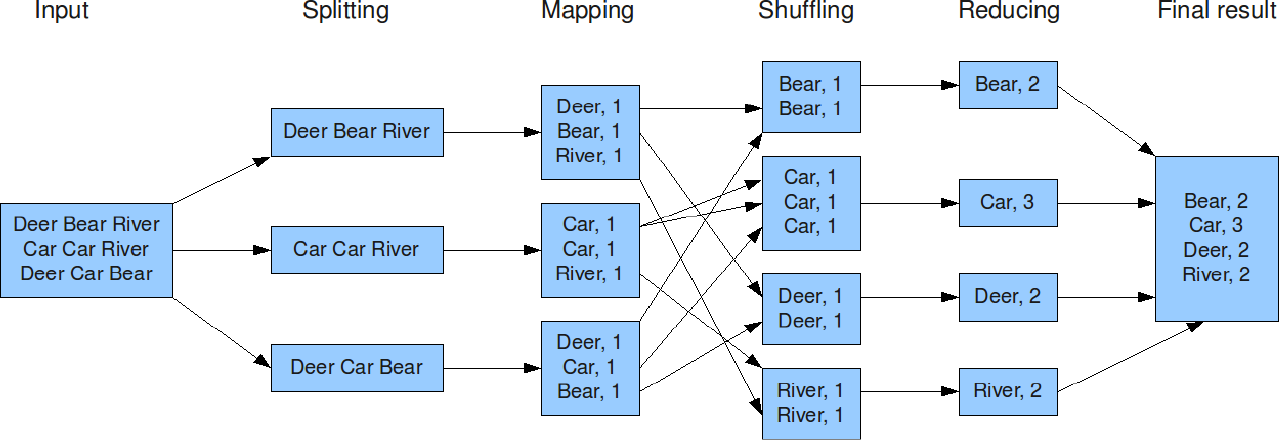
\includegraphics[scale=1.0]{images/map-reduce.png} 
\end{figure}	

\end{frame}

\begin{frame}

A MapReduce framework is generally composed of these operations:
\vspace*{0.6em}

\begin{itemize}
	\item{\textbf{Split}: Divides the input data into parallel streams to provide the cluster nodes (only needed if data already stored)}
	\item{\textbf{Read}: Reads the data streams by splitting them into units to be process (for a text file: 1 unit =  1 line)}
	\item{\textbf{Map}\footnotemark[1]: Each worker node applies the map function to the local data and writes the output to temporary storage (the result of which is stored in <key,value> pairs)}
	\item{\textbf{Shuffle}: Worker nodes redistribute data according to the output keys (produced by the map function) so that all data belonging to a key is on the same worker node}
	\item{\textbf{Reduce}\footnotemark[1]: The worker nodes now process each group of output data by key in parallel}
\end{itemize} 
\vspace*{0.6em}

\footnotetext[1]{Map and Reduce: the most important operations}
\end{frame}
\begin{frame}[fragile]

Developers are \textbf{responsible to develop the mapper and the reducer} (sometimes a \textbf{combiner} to "pre-reduce data" before mapping as well).
\vspace*{0.6em}

The following pseudo-code describes a mapper and a reducer for counting distinct words in a massive text:
\vspace*{0.6em}

\begin{verbatim}
Map(String input_key, String input_values) :
   foreach word w in input_values:
      EmitIntermediate( w, "‘1"’);
Reduce (String key, Iterator intermediate_values):
   int result=0;
   foreach v in intermediate_values:
      result += ParseInt( v );
      Emit( key, String( result ));
\end{verbatim}

\begin{block}{The main Hadoop programming language}
On Hadoop  mappers and reducers are coded in the \textbf{Java programming language}
\end{block}

\end{frame}
\begin{frame}

Now let's see a real example of a \textbf{mapper} and a \textbf{reducer} coded in Java\footnote{You can find the corresponding example here: https://www.guru99.com/create-your-first-hadoop-program.html}. The goal here is to count distinct countries.
\vspace*{0.6em}



	\begin{figure}
	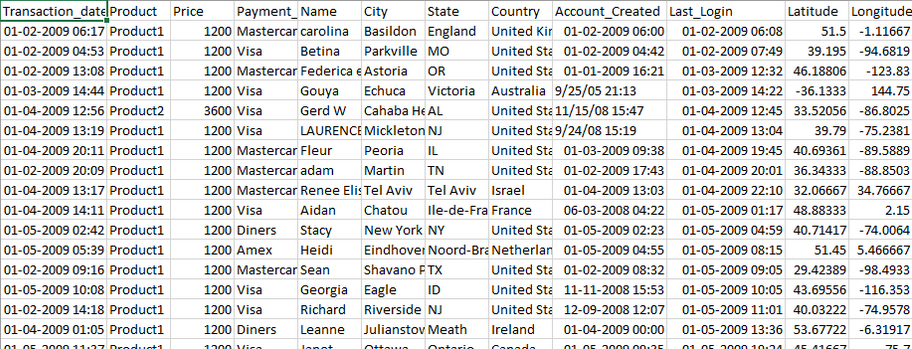
\includegraphics[scale=1.5]{images/hadoop-example-1.png} 
	\caption{Sample of all the data contained in the HDFS (presented as columns)}
	\end{figure}	

\end{frame}
\begin{frame}[fragile]

The mapper of this example (see the content lines 15 to 17):
\vspace*{0.6em}

\begingroup
\fontsize{6pt}{10pt}\selectfont
\begin{Verbatim}[numbers=left,xleftmargin=5mm]
package SalesCountry;

import java.io.IOException;

import org.apache.hadoop.io.IntWritable;
import org.apache.hadoop.io.LongWritable;
import org.apache.hadoop.io.Text;
import org.apache.hadoop.mapred.*;

public class SalesMapper extends MapReduceBase implements Mapper <LongWritable, Text, Text, IntWritable> {
        private final static IntWritable one = new IntWritable(1);

        public void map(LongWritable key, Text value, OutputCollector <Text, IntWritable> output, 
        Reporter reporter) throws IOException {
                String valueString = value.toString();
                String[] SingleCountryData = valueString.split(",");
                output.collect(new Text(SingleCountryData[7]), one);
        }
}
\end{Verbatim}
\endgroup
\end{frame}
\begin{frame}[fragile]
The reducer of this example (see the content lines 15 to 22):
\vspace*{0.6em}

\begingroup
\fontsize{6pt}{8pt}\selectfont
\begin{Verbatim}[numbers=left,xleftmargin=5mm]
package SalesCountry;

import java.io.IOException;
import java.util.*;

import org.apache.hadoop.io.IntWritable;
import org.apache.hadoop.io.Text;
import org.apache.hadoop.mapred.*;

public class SalesCountryReducer extends MapReduceBase implements Reducer<Text, IntWritable, Text, 
IntWritable> {
        public void reduce(Text t_key, Iterator<IntWritable> values, 
        OutputCollector<Text,IntWritable> output, 
        Reporter reporter) throws IOException {
                Text key = t_key;
                int frequencyForCountry = 0;
                while (values.hasNext()) {
                      // replace type of value with the actual type of our value
                      IntWritable value = (IntWritable) values.next();
                      frequencyForCountry += value.get();                       
                }
                output.collect(key, new IntWritable(frequencyForCountry));
        }
}
\end{Verbatim}
\endgroup

\end{frame}
\begin{frame}
YARN (Yet Another Resource Negotiator) is used in the Hadoop ecosystem launch MapReduce "jobs" coded in Java:
\vspace*{0.6em}

\begin{itemize}
\item{YARN allows to \textbf{manage jobs on a cluster} of machines}
\item{YARN can \textbf{move a process from one machine to another} in case of failure or progress judged too slow}
\item{YARN is \textbf{transparent for the user}}
\item{YARN \textbf{makes sure that it is executed executed as quickly as possible}}
\end{itemize}

\end{frame}
\begin{frame}[fragile]

YARN does the MapReduce:
\vspace*{0.6em}

\begin{enumerate}
\item{At the beginning, YARN \textbf{queries the location of the data from the Namenode} (and decompress on Datanodes)}
\item{YARN \textbf{splits building pairs} to be supplied to the Map tasks}
\item{YARN \textbf{creates Map processes} on each machine containing part of the data}
\item{YARN \textbf{sorts the pairs coming out of Map according to their key} and sends them to the machine running the \textbf{Reduce task concerned by this key}}
\item{The \textbf{Reduce tasks receive a list of pairs and perform the reduction of values} (max, sum, avg...)}
\end{enumerate}

\begin{verbatim}
yarn jar /usr/lib/hadoop-mapreduce/hadoop-streaming.jar \
-files mapper.py,reducer.py \
-mapper mapper.py -reducer reducer.py \
-input livres -output sortie
\end{verbatim}

\end{frame}
\subsection{Pig and Pig Latin}

\begin{frame}
There is an easier way to perform MapReduce jobs: \textbf{PIG} (and \textbf{Pig Latin})
\vspace*{0.6em}

\begin{figure}
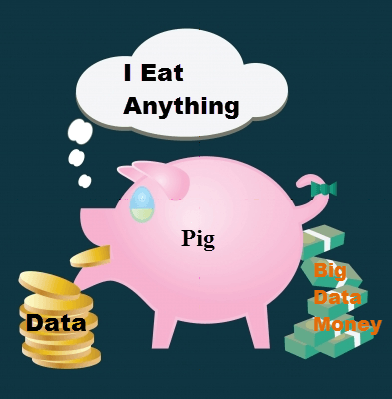
\includegraphics[scale=1.2]{images/pig.png} 
\end{figure}	


Pig was originally created by "Yahoo!". Pig allows to \textbf{write useful treatments on data without undergoing the complexity of Java}. 

\begin{block}{Pig's goal}
The goal is to make Hadoop accessible to people that are not Computer Science scientists: physicists, statisticians, mathematicians...
\end{block}

\end{frame}
\begin{frame}

Differences between Pig and Hadoop MapReduce:
\vspace*{0.6em}

\begin{center}
	\resizebox{\columnwidth}{!}{
	\begin{tabular}{ m{5cm} | m{5cm} }
	\textbf{Pig} & \textbf{Hadoop MapReduce} \\ \hline
	Data flow language & Data processing framework \\ \hline
	High-level language & Low-level and rigid \\ \hline
	Can easily perform a Join & Perform join between datasets very difficult \\ \hline
    Basic knowledge of SQL is enough for Apache Pig & Need to be familiar with Java \\ \hline
    Use a multi-query approach  & Require almost 20 times more code for same task \\ \hline
	No need for compilation & Go through a long compilation process \\ 
	\end{tabular}
	}
	\end{center}

\end{frame}
\begin{frame}
There are some similarities between SQL and Pig Latin (common keywords: JOIN, ORDER, LIMIT...) but their principle is different:
\vspace*{0.6em}

\begin{itemize} 
\item{\textbf{In SQL}: You \textbf{build queries that describe the data to obtain}. We don't know how the SQL engine will calculate the result. We only know that internally, the query will be broken down into loops and comparisons on the data and making the best use of the indexes}
\item{\textbf{In Pig Latin}: We \textbf{build programs that contain the explicit instructions}. We describe exactly how the result should be obtained, what calculations should be result is to be obtained, what calculations are to be made and in what order.}
\end{itemize}

\end{frame}

\begin{frame}

\begin{itemize}
\item{A Pig Latin program consists of \textbf{a series of transformations to apply to input data} to produce output data}
\item{\textbf{These operations describe a data flow}, translated into an executable representation}
\item{Underneath, \textbf{these transformations are actually performed by series of hidden MapReduce jobs}}
\item{Pig allows the programmer to \textbf{focus on data} rather than the nature of execution}
\item{Pig Latin is a \textbf{relatively easy language} using familiar keywords from data processing (Join, Group, Filter, etc)}
\end{itemize}

\end{frame}

\begin{frame}

\begin{columns}[c]
\column{.4\textwidth}	
\begin{figure}
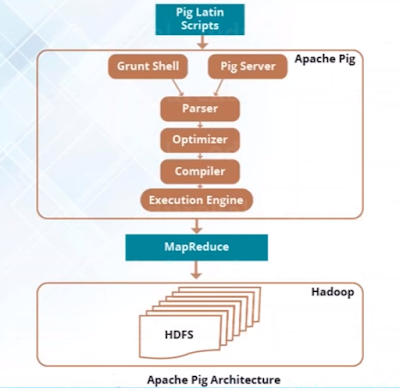
\includegraphics[scale=1.5]{images/pig-latin-chart.png} 
\end{figure}	

\column{.6\textwidth}	
\begin{itemize}
\item{\textbf{Pig Latin}: Series of transformations applied to input data to produce results}
\item{\textbf{Pig Latin Script}: Contains the pig commands in a file (.pig)}
\item{\textbf{Grunt Shell}: Interactive shell for running pig commands}
\item{\textbf{Parser}: Checks the syntax of the script and other miscellaneous checks}
\item{\textbf{Optimizer}: Carries out the logical optimizations}
\item{\textbf{Compiler}: Compiles the optimized logical plan into a series of MapReduce jobs}
\item{\textbf{Execution Engine}: Submits MapReduce jobs to Hadoop in a sorted order}
\end{itemize}



\end{columns}
	

\end{frame}
\begin{frame}
The Pig Latin data model:
\vspace*{0.6em}

\begin{columns}[c]
\column{.4\textwidth}	

\begin{figure}
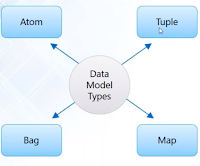
\includegraphics[scale=2.2]{images/pig-data-model.png} 
\end{figure}	

\column{.6\textwidth}	
\begin{itemize}
\item{\textbf{Atom}: Any single value in Pig Latin, stored as string and can be used as string and number (Ex: 1, 'a', 34)}
\item{\textbf{Tuple}: Similar to a row in a table of relational database (Ex: ("Jean", 35, "Teacher"))}
\item{\textbf{Bag}: Unordered set of tuples (Ex: {(1,Linkin Park,7,California), (Metalica,8),(Mega Death,5,Los Angeles)})}
\item{\textbf{Map}: A set of key-value pairs (Ex: Jean\#37)}
\item{\textbf{Relation}: A bag of tuples...}
\end{itemize}

\end{columns}


\end{frame}
\begin{frame}
Introduction to Pig Latin:
\vspace*{0.6em}

Language providing \textbf{statements} as basic constructs which include \textbf{expressions}, \textbf{schemas} and \textbf{ends with a semicolon} (;)
\vspace*{0.6em}

In general (expect for the LOAD and STORE operations), Pig Latin statements \textbf{take a relation as input and produce another relation as output}
\vspace*{0.6em}

\begin{block}{Notes}
\begin{itemize}
\item{When entering a LOAD statement in the Grunt shell: a semantic check of Pig Latin is carried out}
\item{To see schema of loaded content: DESCRIBE (see content: DUMP)}
\item{See more operators below...}
\end{itemize}
\end{block}
\end{frame}
\begin{frame}

List of relational operators of Pig Latin:
\vspace*{0.6em}

\textbf{Loading and Storing}

\begin{center}
	\resizebox{\columnwidth}{!}{
	\begin{tabular}{ c | m{8cm} }
LOAD & Load the data from HDFS into a relation \newline {\tiny Relation\_Name = LOAD A\_File\_Path USING A\_Function as schema; \newline (Functions can be: BinStorage, JsonLoader, PigStorage, TextLoader)} \\ \hline
STORE &  Save a relation to HDFS \newline {\tiny STORE Relation\_Name INTO A\_File\_Path [USING A\_Function];} \\

	\end{tabular}
	}
\end{center}

\end{frame}
\begin{frame}

\textbf{Filtering}

\begin{center}
	\resizebox{\columnwidth}{!}{
	\begin{tabular}{ c | m{8cm} }
	FILTER & Remove unwanted rows from a relation \newline {\tiny Relation\_Name\_2 = FILTER Relation\_Name BY (condition);} \\ \hline
	DISTINCT & Remove duplicate rows from a relation \newline {\tiny Relation\_Name\_2 = DISTINCT Relatin\_Name;} \\  \hline
	FOREACH, GENERATE & Generate data transformations based on columns of data \newline {\tiny Relation\_name\_2 = FOREACH Relatin\_Name GENERATE (required data);} \\ \hline
	STREAM & Transform a relation using an external program \\ 
	\end{tabular}
	}
\end{center}
	
\end{frame}

\begin{frame}

\textbf{Grouping and Joining}

\begin{center}
	\resizebox{\columnwidth}{!}{
	\begin{tabular}{ c | m{8cm} }
	JOIN & Join two or more relations \newline {\tiny Relation\_Name = JOIN Relation\_1 BY Field\_A, Relation\_2 BY Field\_B;} \\ \hline
	COGROUP & Group the data in two or more relations \newline {\tiny Cogroup\_Data = COGROUP Field\_B by Field\_A, Field\_C by Field\_A;} \\ \hline
	GROUP & Group the data in a single relation \newline {\tiny Group\_data = GROUP Relation\_name BY age;} \\ \hline
	CROSS & Create the cross product of two or more relations \newline {\tiny Relation\_C = CROSS Relation\_A, Relation\_B; } \\
	\end{tabular}
	}
\end{center}

\end{frame}
\begin{frame}

\textbf{Sorting}
\vspace*{0.6em}

\begin{center}
	\resizebox{\columnwidth}{!}{
	\begin{tabular}{ c | m{8cm} }
ORDER & Arrange a relation in a sorted order based on one or more fields (ascending or descending) \newline {\tiny Relation\_2 = ORDER Relation\_1 BY [ASC|DESC] Field\_A;} \\ \hline
LIMIT & Get a limited number of tuples from a relation \newline {\tiny Relation\_2 = LIMIT Relation\_1 N; } \\
	\end{tabular}	
	}
\end{center}
\vspace*{0.6em}
	
\textbf{Combining and Splitting}
\vspace*{0.6em}

\begin{center}
	\resizebox{\columnwidth}{!}{
	\begin{tabular}{ c | m{8cm} }
UNION & Combine two or more relations into a single relation \newline {\tiny Relation\_C = UNION Relation\_A, Relation\_B;} \\ \hline
SPLIT & Split a single relation into two or more relations \newline {\tiny SPLIT Relation\_1 INTO Relation\_2 IF expression,} \\ 	
	\end{tabular}
	
	
	}
\end{center}



\end{frame}

\begin{frame}

\textbf{Diagnostic Operators}


\begin{center}
	\resizebox{\columnwidth}{!}{
	\begin{tabular}{ c | m{8cm} }
	DUMP & Print the content of a relation on the console \newline {\tiny dump Relation\_Name;} \\ \hline
	DESCRIBE & Describe the schema of a relation \newline {\tiny describe Relation\_name;} \\ \hline
	EXPLAIN & View the logical, physical or MapReduce execution plans to compute a relation \newline {\tiny explain Relation\_name;} \\ \hline
	ILLUSTRATE & View the step-by-step execution of a series of statements \newline {\tiny illustrate Relation\_name;}  \\ 
	\end{tabular}
	}
	\end{center}


\end{frame}
\subsection{Examples of Pig commands}
\begin{frame}[fragile]
Imagine we have a dept.csv file stored on HDFS, here load it and perform some basic actions on the data:
\vspace*{0.6em}
\begingroup
\fontsize{6pt}{10pt}\selectfont
\begin{verbatim}
grunt> dept = LOAD '/pig/dept.csv' USING PigStorage(',') as (deptno:int,dname:chararray,loc:chararray);
grunt> dump dept;
(10,ACCOUNTING,NEW YORK)
(20,RESEARCH,DALLAS)
(30,SALES,CHICAGO)
(40,OPERATIONS,BOSTON)
grunt> describe dept;
dept: {deptno: int,dname: chararray,loc: chararray}
\end{verbatim}
\endgroup

Let's group the data and see what we get:

\begingroup
\fontsize{6pt}{10pt}\selectfont
\begin{verbatim}
grunt> group_multiple = group dept by (deptno,dname);
grunt> dump group_multiple;
((10,ACCOUNTING),{(10,ACCOUNTING,NEW YORK)})
((20,RESEARCH),{(20,RESEARCH,DALLAS)})
((30,SALES),{(30,SALES,CHICAGO)})
((40,OPERATIONS),{(40,OPERATIONS,BOSTON)})
\end{verbatim}
\endgroup

\end{frame}
\begin{frame}[fragile]
Here we perform a JOIN operation:
\vspace*{0.6em}
\begingroup
\fontsize{6pt}{10pt}\selectfont
\begin{verbatim}
grunt> e1 = load '/pig/emp.csv' using PigStorage(',') as
(EMPNO:int,ENAME:chararray,JOB:chararray,MGR:int,HIREDATE:datetime,SAL:int,COMM:int,DEPTNO:int);
grunt> e2 = load '/pig/emp2.csv' using PigStorage(',') as 
(EMPNO:int,ENAME:chararray,JOB:chararray,MGR:int,HIREDATE:datetime,SAL:int,COMM:int,DEPTNO:int);
grunt> emp_join = JOIN e1 BY EMPNO, e2 BY MGR;
grunt> dump emp_join;
(7566,JONES,MANAGER,7839,,2975,,20,7788,SCOTT,ANALYST,7566,,3000,,20)
(7566,JONES,MANAGER,7839,,2975,,20,7902,FORD,ANALYST,7566,,3000,,20)
(7698,BLAKE,MANAGER,7839,,2850,,30,7654,MARTIN,SALESMAN,7698,,1250,1400,30)
(7698,BLAKE,MANAGER,7839,,2850,,30,7900,JAMES,CLERK,7698,,950,,30)
(7698,BLAKE,MANAGER,7839,,2850,,30,7521,WARD,SALESMAN,7698,,1250,500,30)
\end{verbatim}
\endgroup

\end{frame}
\begin{frame}[fragile]
Now we filter the data:

\vspace*{0.6em}
\begingroup
\fontsize{6pt}{10pt}\selectfont
\begin{verbatim}
grunt> filter_emp = FILTER emp BY JOB == 'CLERK';
grunt> dump filter_emp;
(7369,SMITH,CLERK,7902,,800,,20)
(7876,ADAMS,CLERK,7788,,1100,,20)
(7900,JAMES,CLERK,7698,,950,,30)
(7934,MILLER,CLERK,7782,,1300,,10)
\end{verbatim}
\endgroup

We reorder data:
\vspace*{0.6em}
\begingroup
\fontsize{6pt}{10pt}\selectfont
\begin{verbatim}
grunt> order_by_data = ORDER dept BY loc ASC;
grunt> dump order_by_data
(40,OPERATIONS,BOSTON)
(30,SALES,CHICAGO)
(20,RESEARCH,DALLAS)
(10,ACCOUNTING,NEW YORK)
\end{verbatim}
\endgroup

We store the data:
\vspace*{0.6em}
\begingroup
\fontsize{6pt}{10pt}\selectfont
\begin{verbatim}
grunt> store dept into '/dump.txt' using PigStorage(',');
\end{verbatim}
\endgroup

\end{frame}
\begin{frame}
Pig also comes with a set of User Defined Functions (UDFs)

\begin{center}
	\resizebox{\columnwidth}{!}{
	\begin{tabular}{ c | m{7cm} }
AVG() & Computes average of numeric values \\ \hline
PigStorage() & Load and store data as structured text files \\ \hline
TextLoader() & Load unstructured data in UTF-8 format \\ \hline
BinStorage() & Load and store the data in machine readable format \\ \hline
TOBAG() & Convert expressions to individual tuples (placed in a bag) \\ \hline
TOTUPLE() & Convert one or more expressions to tuple \\ \hline
TOMAP() & Convert the key-value pairs into a Map \\ 
\end{tabular}
}
\end{center}

\begin{block}{Note}
Pig Latin is a complete langage! And mastering Pig Latin is not the objective of this course, if you want to know more about it, you can go to this website: http://pig.apache.org/docs/r0.17.0/
\end{block}


\end{frame}
\subsection{Hadoop: pros and cons}

\begin{frame}
Hadoop Pros and Cons
\vspace*{0.6em}

\textbf{Pros}

\begin{itemize}
\item{\textbf{Cost}: Hadoop is \textbf{open-source and uses cost-effective commodity hardware which provides a cost-efficient model}}
\item{\textbf{Scability}: Hadoop is a \textbf{highly scalable model}. A large amount of data is divided into multiple inexpensive machines in a cluster which is processed parallelly}
\item{\textbf{Flexibility}: Hadoop is designed in such a way that it can \textbf{deal with any kind of dataset} like \textbf{structured} (MySQL Data), \textbf{Semi-Structured} (XML, JSON), \textbf{Un-structured} (Images and Videos) efficiently}
\item{\textbf{Speed}: With Hadoop you \textbf{can easily access TBs of data} in just a few minutes}
\item{\textbf{Fault tolerance}: Hadoop uses commodity hardware which can be crashed at any moment: \textbf{data is then replicated} on various DataNodes}
\end{itemize}


\end{frame}


\begin{frame}

\textbf{Cons}

\begin{itemize}
\item{\textbf{Problem with small files}: Hadoop stores the file in the form of file blocks which are from 128MB in size (by default) to 256MB. This \textbf{so many small files surcharge the Namenode and make it difficult to work}}
\item{\textbf{Lots of disk access}: In Hadoop, \textbf{intermediary data results are often read or write to/from the disk} leading to some slowlessness and inefficiency}
\item{\textbf{Vulnerability}: Although is everything for an organization, by default \textbf{the security feature in Hadoop is made un-available}}
\item{\textbf{Difficulty}: Hadoop requires you \textbf{learn to write specific Java MapReduce routines or Pig Latin commands}}
\end{itemize}

\end{frame}

\section{Spark}
\subsection{What is Spark?}

\begin{frame}

	\begin{figure}
	
\includegraphics[scale=1.3]{images/spark_logo.png} 
	\end{figure}	

What is Spark?
\vspace*{0.6em}

\begin{itemize}
\item{Spark is a \textbf{unified analytics engine for large-scale data processing}}
\item{Which is \textbf{10 to 100x faster than Hadoop MapReduce}}
\end{itemize}

\begin{figure}
	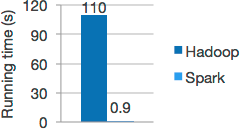
\includegraphics[scale=0.3]{images/spark-comparison.png} 
	\caption{Logistic regression comparison Hadoop MapReduce VS Spark}
\end{figure}	





\end{frame}

\begin{frame}

\begin{itemize}
	\item{Spark is \textbf{also uses a cluster of nodes for computation} (here worker=DataNote, master node=Namenode)}
	\item{Spark applications run as independent sets of processes on a cluster \textbf{coordinated by the SparkContext object} in your main program (called the driver program)}
\end{itemize}

\begin{figure}
	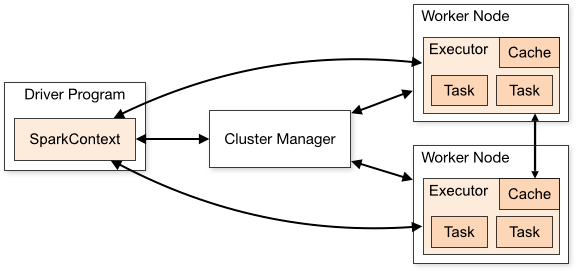
\includegraphics[scale=0.4]{images/sparkcontext.png} 
\end{figure}	
	
\end{frame}

\begin{frame}
	\begin{enumerate}
	\item{The SparkContext \textbf{can connect to several types of cluster managers} to allocate resources (Spark’s own cluster manager, Mesos or even YARN)}
	\item{Once connected, Spark acquires executors on nodes in the cluster, \textbf{running computations and storing data for your application}. Once acquired, \textbf{application code} (defined by JAR or Python files passed to SparkContext) is \textbf{sent to the executors}}
	\item{Finally, the \textbf{SparkContext sends tasks to the executors to run}...}
	\end{enumerate}

\end{frame}



\subsection{Comparison with Hadoop MapReduce}

\begin{frame}
Spark overcomes some of the biggest limitations of Hadoop:
\vspace*{0.6em}

\begin{itemize}
\item{Spark is potentially up \textbf{10 to 100 times faster} than Hadoop MapReduce}
\item{Spark \textbf{utilizes RAM, intermediary data is not stored on disk} 
\begin{itemize}
\item{Hadoop stores a lot of intermediary data on disks for computation}
\end{itemize}}

\item{Spark \textbf{works well for smaller data-sets that can all fit into the RAM} 
\begin{itemize}
\item{Hadoop is \textbf{more effective for truly massive datasets}}
\end{itemize}
}
\item{Spark is more popular than Hadoop MapReduce 
\begin{itemize}
\item{Spark is \textbf{easier to learn} and you can use \textbf{Python and Scala with it}}
\end{itemize}}
\end{itemize}
 

\end{frame}


\begin{frame}
Reasons why Spark is s much faster than Hadoop MapReduce:
\vspace*{0.6em}

\begin{itemize}
\item{Spark provides \textbf{in-memory computation} (designed to \textbf{transform data in-memory and hence reduces computation time}. While MapReduce writes/read a lot of intermediate results back and forth to/from Disk}
\item{Spark utilizes \textbf{Direct Acyclic Graph} that \textbf{helps to do all the optimization and computation in a single stage} rather than multiple stages in the MapReduce model}
\item{\textbf{Spark core is developed using the SCALA programming language} which is faster than JAVA}
\end{itemize}

\end{frame}

\subsection{Spark's Resilient Distributed Dataset (RDDs)}



\begin{frame}

RDD (Resilient Distributed Dataset) is the \textbf{fundamental data structure of Spark} which are an \textbf{immutable}\footnote{An immutable object is an object whose internal state remains constant after it has been entirely created} collection of objects which computes on the different node of the cluster. 
\vspace*{0.6em}

Decomposing the name RDD:
\vspace*{0.6em}

\begin{itemize}
\item{\textbf{Resilient}: \textbf{fault-tolerant with the help of RDD lineage graph (DAG)} and so able to recompute missing or damaged partitions due to node failures}
\item{\textbf{Distributed}: Data \textbf{resides on multiple nodes} (as partitions of RDD)}
\item{\textbf{Dataset}: Records of the data you work with. The user can load the data set externally which can be either \textbf{JSON file, CSV file, text file or database via JDBC with no specific data structure}}
\end{itemize}

\end{frame}

\begin{frame}

As mentioned above, \textbf{each and every dataset in Spark RDD is logically partitioned across many servers} so that they can be computed on different nodes of the cluster. 
\vspace*{0.6em}

\begin{figure}
	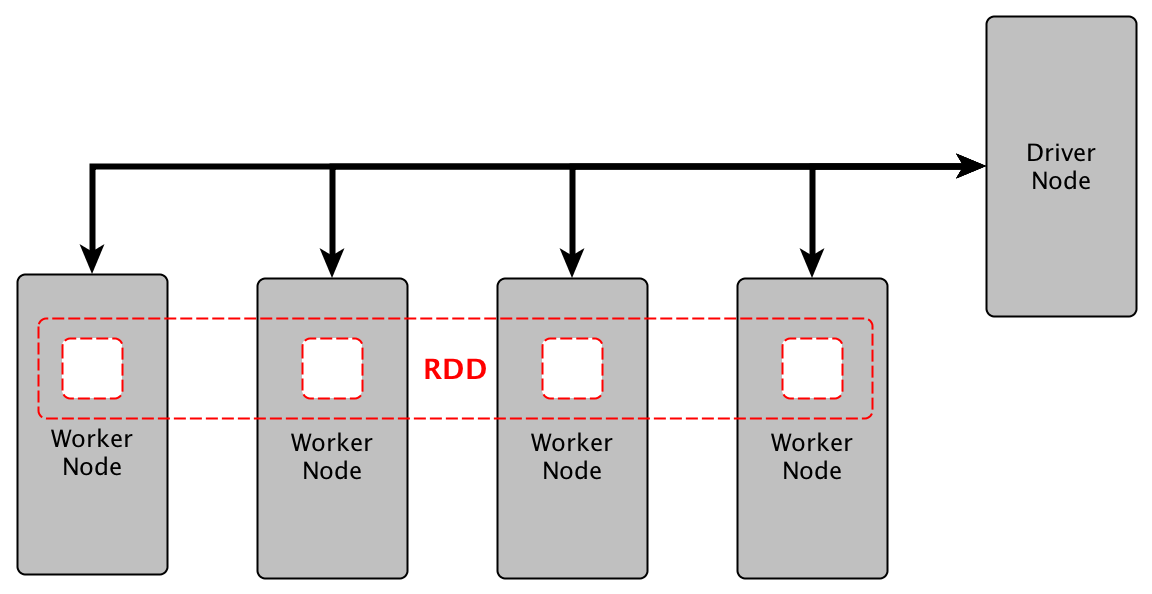
\includegraphics[scale=0.2]{images/rdd_partitions.png} 
\end{figure}	
	
\end{frame}

\begin{frame}

\begin{figure}
	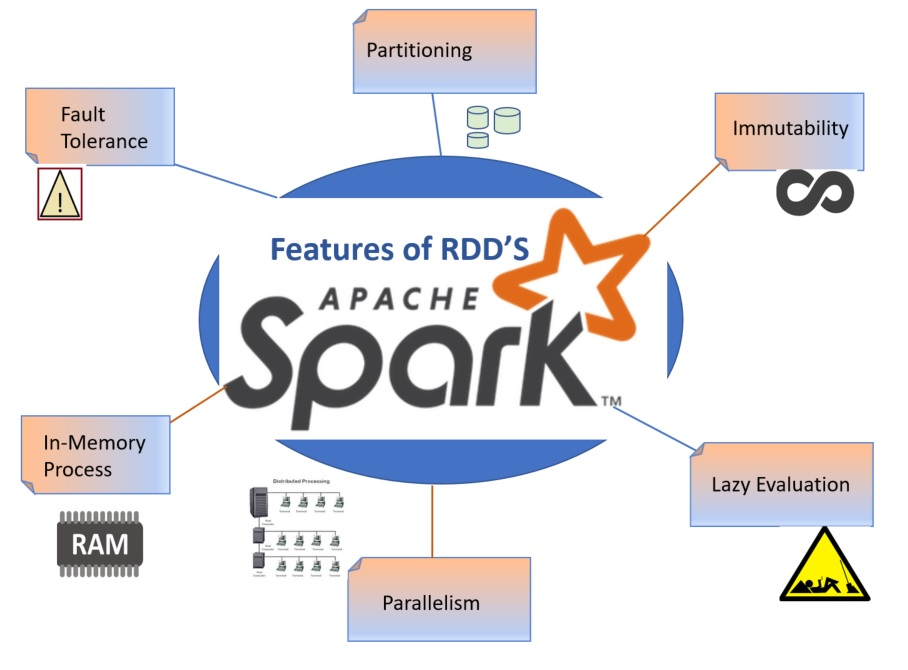
\includegraphics[scale=0.5]{images/featuresofrdd.jpg} 
\end{figure}	
	
\end{frame}

\begin{frame}
Main features of RDD:
\vspace*{0.6em}

\begin{itemize}
\item{\textbf{In-memory Computation}: Intermediate results are stored in distributed memory (RAM) instead of stable storage (disk)}
\item{\textbf{Lazy Evaluations}: All \textbf{transformations in Spark are lazy} the results are not calculated right away. Instead, they \textbf{just remember the transformations to apply}. Spark \textbf{only computes the transformations when an action requires a result for the driver program}}
\item{\textbf{Fault Tolerance}: Spark RDDs are fault tolerant as they \textbf{track data lineage information to rebuild lost data} automatically on failure}
\item{\textbf{Partitioning}: Partition is \textbf{the fundamental unit of parallelism in Spark RDD}. Each partition is one logical division of data which is mutable. One can create a partition through some transformations on existing partitions}
\item{\textbf{Immutability}: Data is \textbf{safe to share across processes}. It can also be created or retrieved anytime which makes caching, sharing and replication easy}
\end{itemize}

\end{frame}

\begin{frame}

More information about the Fault Tolerance feature of RDD:
\vspace*{0.6em}

The \textbf{RDD data lineage is stored in the master node of the cluster} and allow to \textbf{restart the processing from everywhere} in case of problem:
\vspace*{0.6em}

\begin{figure}
	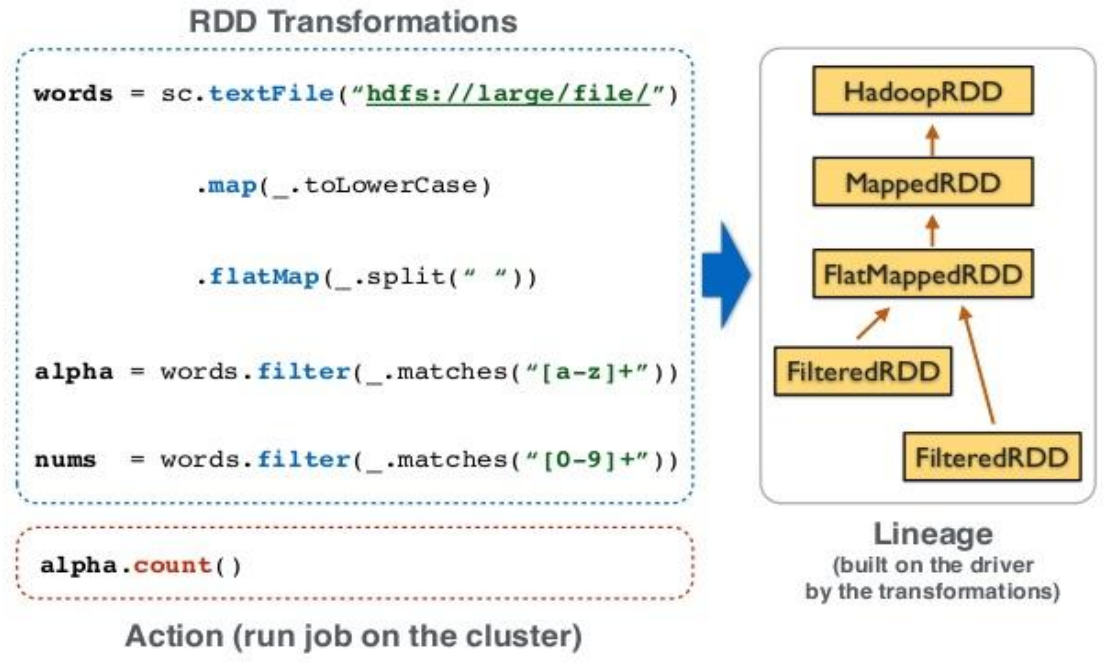
\includegraphics[scale=0.25]{images/rdd_lineage.png} 
\end{figure}

\end{frame}

\subsection{PySpark: Spark with Python!}
\begin{frame}[fragile]

Here is a very brief introduction to PySpark... We will start with a very simple example with this piece of code:
\vspace*{0.6em}

\begin{verbatim}
from pyspark import SparkConf, SparkContext
nomappli = "name1"
config = SparkConf().setAppName(nameppli)
config.setMaster("spark://master:7077")
sc = SparkContext(conf=config)
\end{verbatim}

\begin{itemize}
\item{"sc" represents the SparkContext}
\item{It is an object that has several methods including those that create RDDs}
\item{The commented line config.setMaster() allows to define the URL of the Spark Master}
\end{itemize}

\end{frame}
\begin{frame}[fragile]
Now that the SparkContext is ready, we can create a very simple RDD:
\vspace*{0.6em}

\begin{verbatim}
nums=sc.parallelize([1,2,3,4]) 
\end{verbatim} 

Now we apply a transformation to the data with a lambda function (to compute the square of nums), it is a map transformation:
\vspace*{0.6em}

\begin{verbatim}
squared = nums.map(lambda x: x*x).collect()
for num in squared:
    print('%i ' % (num))
1 
4 
9 
16 
\end{verbatim}
\end{frame}
\begin{frame}[fragile]

A more convenient way to process the data with PySpark is to use a DataFrame and use \textbf{Spark SQL} (SQLContext is used to initiate the functionalities of Spark SQL): 
\vspace*{0.6em}

\begin{verbatim}
sqlContext = SQLContext(sc)
list_p=[('John',19),('Smith',29),('Adam',35),('Henry',50)]
rdd = sc.parallelize(list_p) 
rdd.map(lambda x: Row(name=x[0], age=int(x[1])))  
sqlContext.createDataFrame(ppl)
list_p = [('John',19),('Smith',29),('Adam',35),('Henry',50)]
rdd = sc.parallelize(list_p)
ppl = rdd.map(lambda x: Row(name=x[0], age=int(x[1])))
DF_ppl = sqlContext.createDataFrame(ppl)  
DF_ppl.printSchema()
root
 |-- age: long (nullable = true)
 |-- name: string (nullable = true)
\end{verbatim}



\end{frame}
\begin{frame}[fragile]
Here is the counting words example with PySpark:
\begingroup
\fontsize{6pt}{10pt}\selectfont
\begin{verbatim}
import sys
from pyspark import SparkContext

sc = SparkContext()
lines = sc.textFile(sys.argv[1])
word_counts = lines.flatMap(lambda line: line.split(' ')) \
                   .map(lambda word: (word, 1)) \
                   .reduceByKey(lambda count1, count2: count1 + count2) \
                   .collect()

for (word, count) in word_counts:
    print(word, count)    
\end{verbatim}
\endgroup
Easier than writing a Java Hadoop MapReduce routine, right?

\end{frame}

\begin{frame}

During next TD:

\begin{itemize}
	\item{We will practice Hadoop Pig
		\begin{itemize}
			\item{Make sure you have pulled the corresponding Docker image (apache-pig)!}
		\end{itemize}			
	}
	\item{And we will practice PySpark 
		\begin{itemize}
			\item{Make sure the Docker Compose application with Spark is working}
			\item{Spend some time to get familiar with the PySpark documentation}
		\end{itemize}		
	}
\end{itemize}

\begin{block}{PySpark official documentation}
The official documentation http://spark.apache.org/docs/latest/api/python/getting\_started/index.html
\end{block}

\end{frame}
\end{document}	
	